\let\negmedspace\undefined
\let\negthickspace\undefined
\documentclass[journal]{IEEEtran}
\usepackage[a5paper, margin=10mm, onecolumn]{geometry}
\usepackage{tfrupee} 
\setlength{\headheight}{1cm} 
\setlength{\headsep}{0mm}     

\usepackage{gvv-book}
\usepackage{gvv}
\usepackage{cite}
\usepackage{amsmath,amssymb,amsfonts,amsthm}
\usepackage{algorithmic}
\usepackage{graphicx}
\usepackage{textcomp}
\usepackage{xcolor}
\usepackage{txfonts}
\usepackage{listings}
\usepackage{enumitem}
\usepackage{mathtools}
\usepackage{gensymb}
\usepackage{comment}
\usepackage[breaklinks=true]{hyperref}
\usepackage{tkz-euclide} 
\usepackage{listings}
\def\inputGnumericTable{}                                 
\usepackage[latin1]{inputenc}                                
\usepackage{color}                                            
\usepackage{array}                                            
\usepackage{longtable}                                       
\usepackage{calc}                                             
\usepackage{multirow}                                         
\usepackage{hhline}                                           
\usepackage{ifthen}                                           
\usepackage{lscape}
\usepackage{circuitikz}
\tikzstyle{block} = [rectangle, draw, fill=blue!20, 
    text width=4em, text centered, rounded corners, minimum height=3em]
\tikzstyle{sum} = [draw, fill=blue!10, circle, minimum size=1cm, node distance=1.5cm]
\tikzstyle{input} = [coordinate]
\tikzstyle{output} = [coordinate]
\renewcommand{\thefigure}{\theenumi}
\renewcommand{\thetable}{\theenumi}
\setlength{\intextsep}{10pt} % Space between text and floats
\numberwithin{equation}{enumi}
\numberwithin{figure}{enumi}
\renewcommand{\thetable}{\theenumi}

\begin{document}

\bibliographystyle{IEEEtran}
\vspace{3cm}

\title{2.8.15}
\author{EE25BTECH11032 - Kartik Lahoti}
\maketitle

\subsection*{Question: } 
Find the position vector of a point $\vec{A}$ in space such that $\vec{OA}$ is inclined at $60\degree$ with $\vec{OX}$ and $45\degree$ to $\vec{OY}$ and $\mydet{\vec{OA}} = 10 $units.

\solution 

\subsubsection*{Given }
Let $\vec{A} - \vec{O}$ be represented as $\vec{R}$
\begin{align}
    \norm{\vec{R}} = 10 \text{ , Angle with } x\text{-axis} = 60\degree \text{ and } y\text{-axis } = 45\degree
\end{align}

\begin{align}
    \vec{R} = \norm{\vec{R}} \vec{m} 
\end{align}
where, let $\vec{m}$ be the unit vector in direction of $\vec{R}$. 

\begin{align}
    \vec{m} = \myvec{\cos(60\degree) \\ \cos(45\degree) \\ m_3 }
\end{align}

\begin{align}
    \vec{m}^{\top}\vec{m} = 1
\end{align}
\begin{align}
    \cos^2(60\degree) + \cos^2(45\degree) + m_3^2 &= 1 \\ 
    m_3 &=\pm \frac{1}{2}  
\end{align}

\begin{align}
    \therefore \vec{R} = 10\myvec{\frac{1}{2} \\ \frac{1}{\sqrt{2}} \\ \pm \frac{1}{2}}
\end{align}

Hence , 
\begin{align}
    \vec{A}_1 = \myvec{5 \\ 5\sqrt{2} \\ +5} \text{ and } \vec{A}_2 = \myvec{5 \\ 5\sqrt{2} \\ -5} 
\end{align}
are the position vector for point $\vec{A}$



\begin{figure}[H]
    \centering
    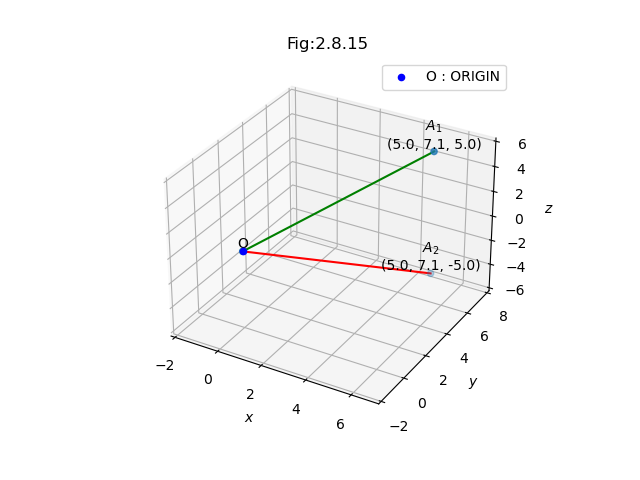
\includegraphics[width=1\columnwidth]{figs/vector1.png}
    \caption*{}
    \label{fig:}
\end{figure}

\end{document}


